\chapter{Methodology} \label{Methodology}

\lhead{Chapter 4. \emph{Methodology}}
In this section, we will cover the implementation details of this project.

First, we will discuss the different neural network architectures then we will discuss the training of these neural networks and finally how we are going to evaluate them.

We are assuming to know the equilibrium. It is a shortcut we are making because a lot of research had been done on equilibrium finding (section: \ref{LR:section:imperfect-game-solving}) and if we assume to know an equilibrium or a partial equilibrium this would help to reduce the input of the neural networks and improve the learning time.

We are aiming to have an algorithm that is universal to every imperfect game. To do so we are relying on notions that are common to all imperfect games, such as equilibrium and the reward of a game.

\section{Neural Network Architecture} \label{methodology:NN}
There will be two neural networks, one that builds the opponent model and one that decides which actions should be taken during a game. I have decided to use two NN because I believe that the opponent modeling NN requires to have the knowledge of a full game. In addition that will allow to have a specific set of information for the input of these NN and so improve the learning speed.

For optimization reasons, we do not want that these neural networks have to learn how the game works. Instead, we will try to process the input feed to these neural networks with the game knowledge. For example, giving the equilibrium of an action instead of giving the info set (the info set is the representation of the public and private information). It is a challenging constraint but we believe that it will enable this NN to scale way better.

\subsection{Opponent modelling NN} \label{methodology:opponent-modelling}
For the opponent modeling neural network, it needs to learn how the opponent play over time. To do that it needs to have multiple knowledge.

\subsubsection{Knowledge of previous games}

It needs to know previous games. It is done by having memory. Either an internal memory such as LSTM (section: \ref{LR:LSTM}) or by having a manual memory which is using information from the output of the neural network as its input. These kinds of neural networks are RNN (section: \ref{LR:RNN}).

\subsubsection{Knowledge about game history} \label{methodology:opponent-modelling:game-history}

It needs to know the game history. The game history consists of the multiple actions that had been done during a game. With a game history, you're supposed to be able to know every step of the game. A simple idea would be to give the different info set and the different actions taken by each player. However as said previously we do not want to feed the info set to the neural network.

Instead our idea is to represent the game history with a succession of:
\begin{itemize}
    \item agent action
    \item opponent action
    \item equilibrium for the opponent action
\end{itemize}

Like this, the game knowledge is encapsulated in the \textit{equilibrium for the opponent action}.

The equilibrium for an opponent's action is not always known. Indeed, to know it we need to have access to the private information of the opponent. In some cases, this information will not be known and we can not ignore this case.

One approach to this problem is to treat the two cases separately \citep{ganzfried2015safe}. However, because we are using a neural network the size and meaning of the input are rigid. That would require having two different neural networks. For the sake of simplicity and optimization reasons, we decide to not treat this.

One thing worth mentioning is that even if we do not know the private information of the opponent we can still use the equilibrium to give game knowledge. Indeed, instead of having a specific equilibrium for the information set, you can have a global equilibrium. For example in poker, if you're the first player you should bet 50\% of the time (the \% is just here, for example, it depends on the poker variant). So, if you notice that the opponent bet only 10\% of the time you can exploit it. It means that this global equilibrium is valuable information.

We decided to represent both of these equilibrium knowledge for the opponent's action. The global equilibrium and the specific equilibrium. If the private information of the opponent is unknown we can not have a specific equilibrium and so will just set the specific equilibrium values to -1 to indicate that no values are available. Figure \ref{fig:opponent-equilibrium}

\begin{figure}[ht]
    \centering
    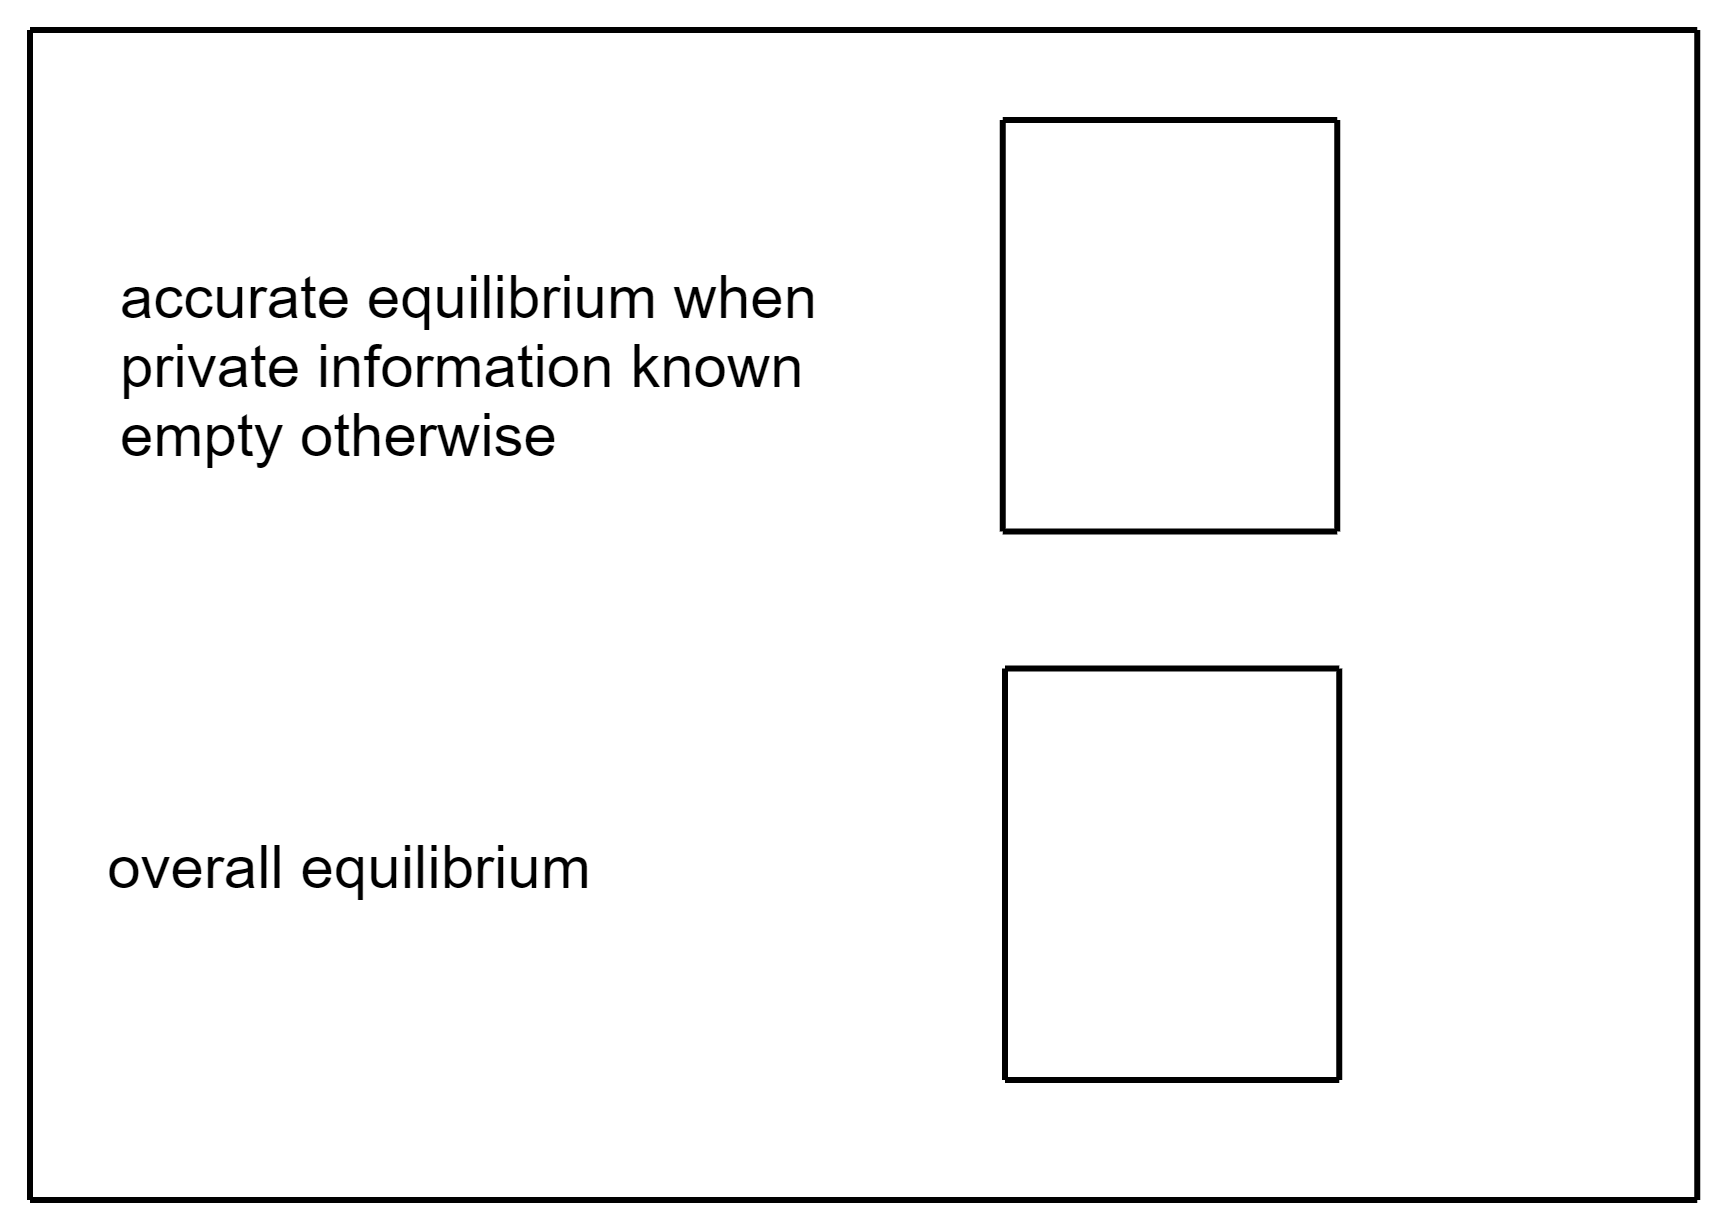
\includegraphics[width=0.7\textwidth]{Figures/opponent-equilibrium.png}
    \caption{Equilibrium for the opponent action}
    \label{fig:opponent-equilibrium}
\end{figure}

Also, another representation that we are thinking of is representing either the specific or the global equilibrium depending if we know the private information of the opponent. And to indicate the NN that it's the specific equilibrium we will have a flag (a binary value) set to 1 if it is the specific equilibrium.

Also to not mess up with the order of the input, if the opponent start we leave empty the first agent action.

Finally, because the input size of NN is constant we can not change the size of the input depending on the number of actions done in the game. To overcome this issue we will left empty a part of the input if the game stopped before.

\subsubsection{Knowledge about game result}

In the effort of feeding up the NN with game knowledge, we believe that the game result is valuable information that will greatly improve the performance of the NN.

The game result is as its name suggests the outcome of the game. For example in poker who won and how much money the player won.

This is the only part of the NN that is game-specific because each game can have valuable outcome information. However, we believe that it is not a problem for the generalization of this algorithm to other imperfect games. Indeed the outcome information is easy to retrieve and in most of the games, it only represents a small set of information.

\subsubsection{Conclusion}

In figure \ref{fig:opponent-modelling-nn-rnn} you can find a sum-up of this information with a RNN architecture where the opponent model also represents the NN memory. In figure \ref{fig:opponent-modelling-nn-lstm} it is the same information however the memory is managed internally as an LSTM would do.

\begin{figure}[ht]
    \centering
    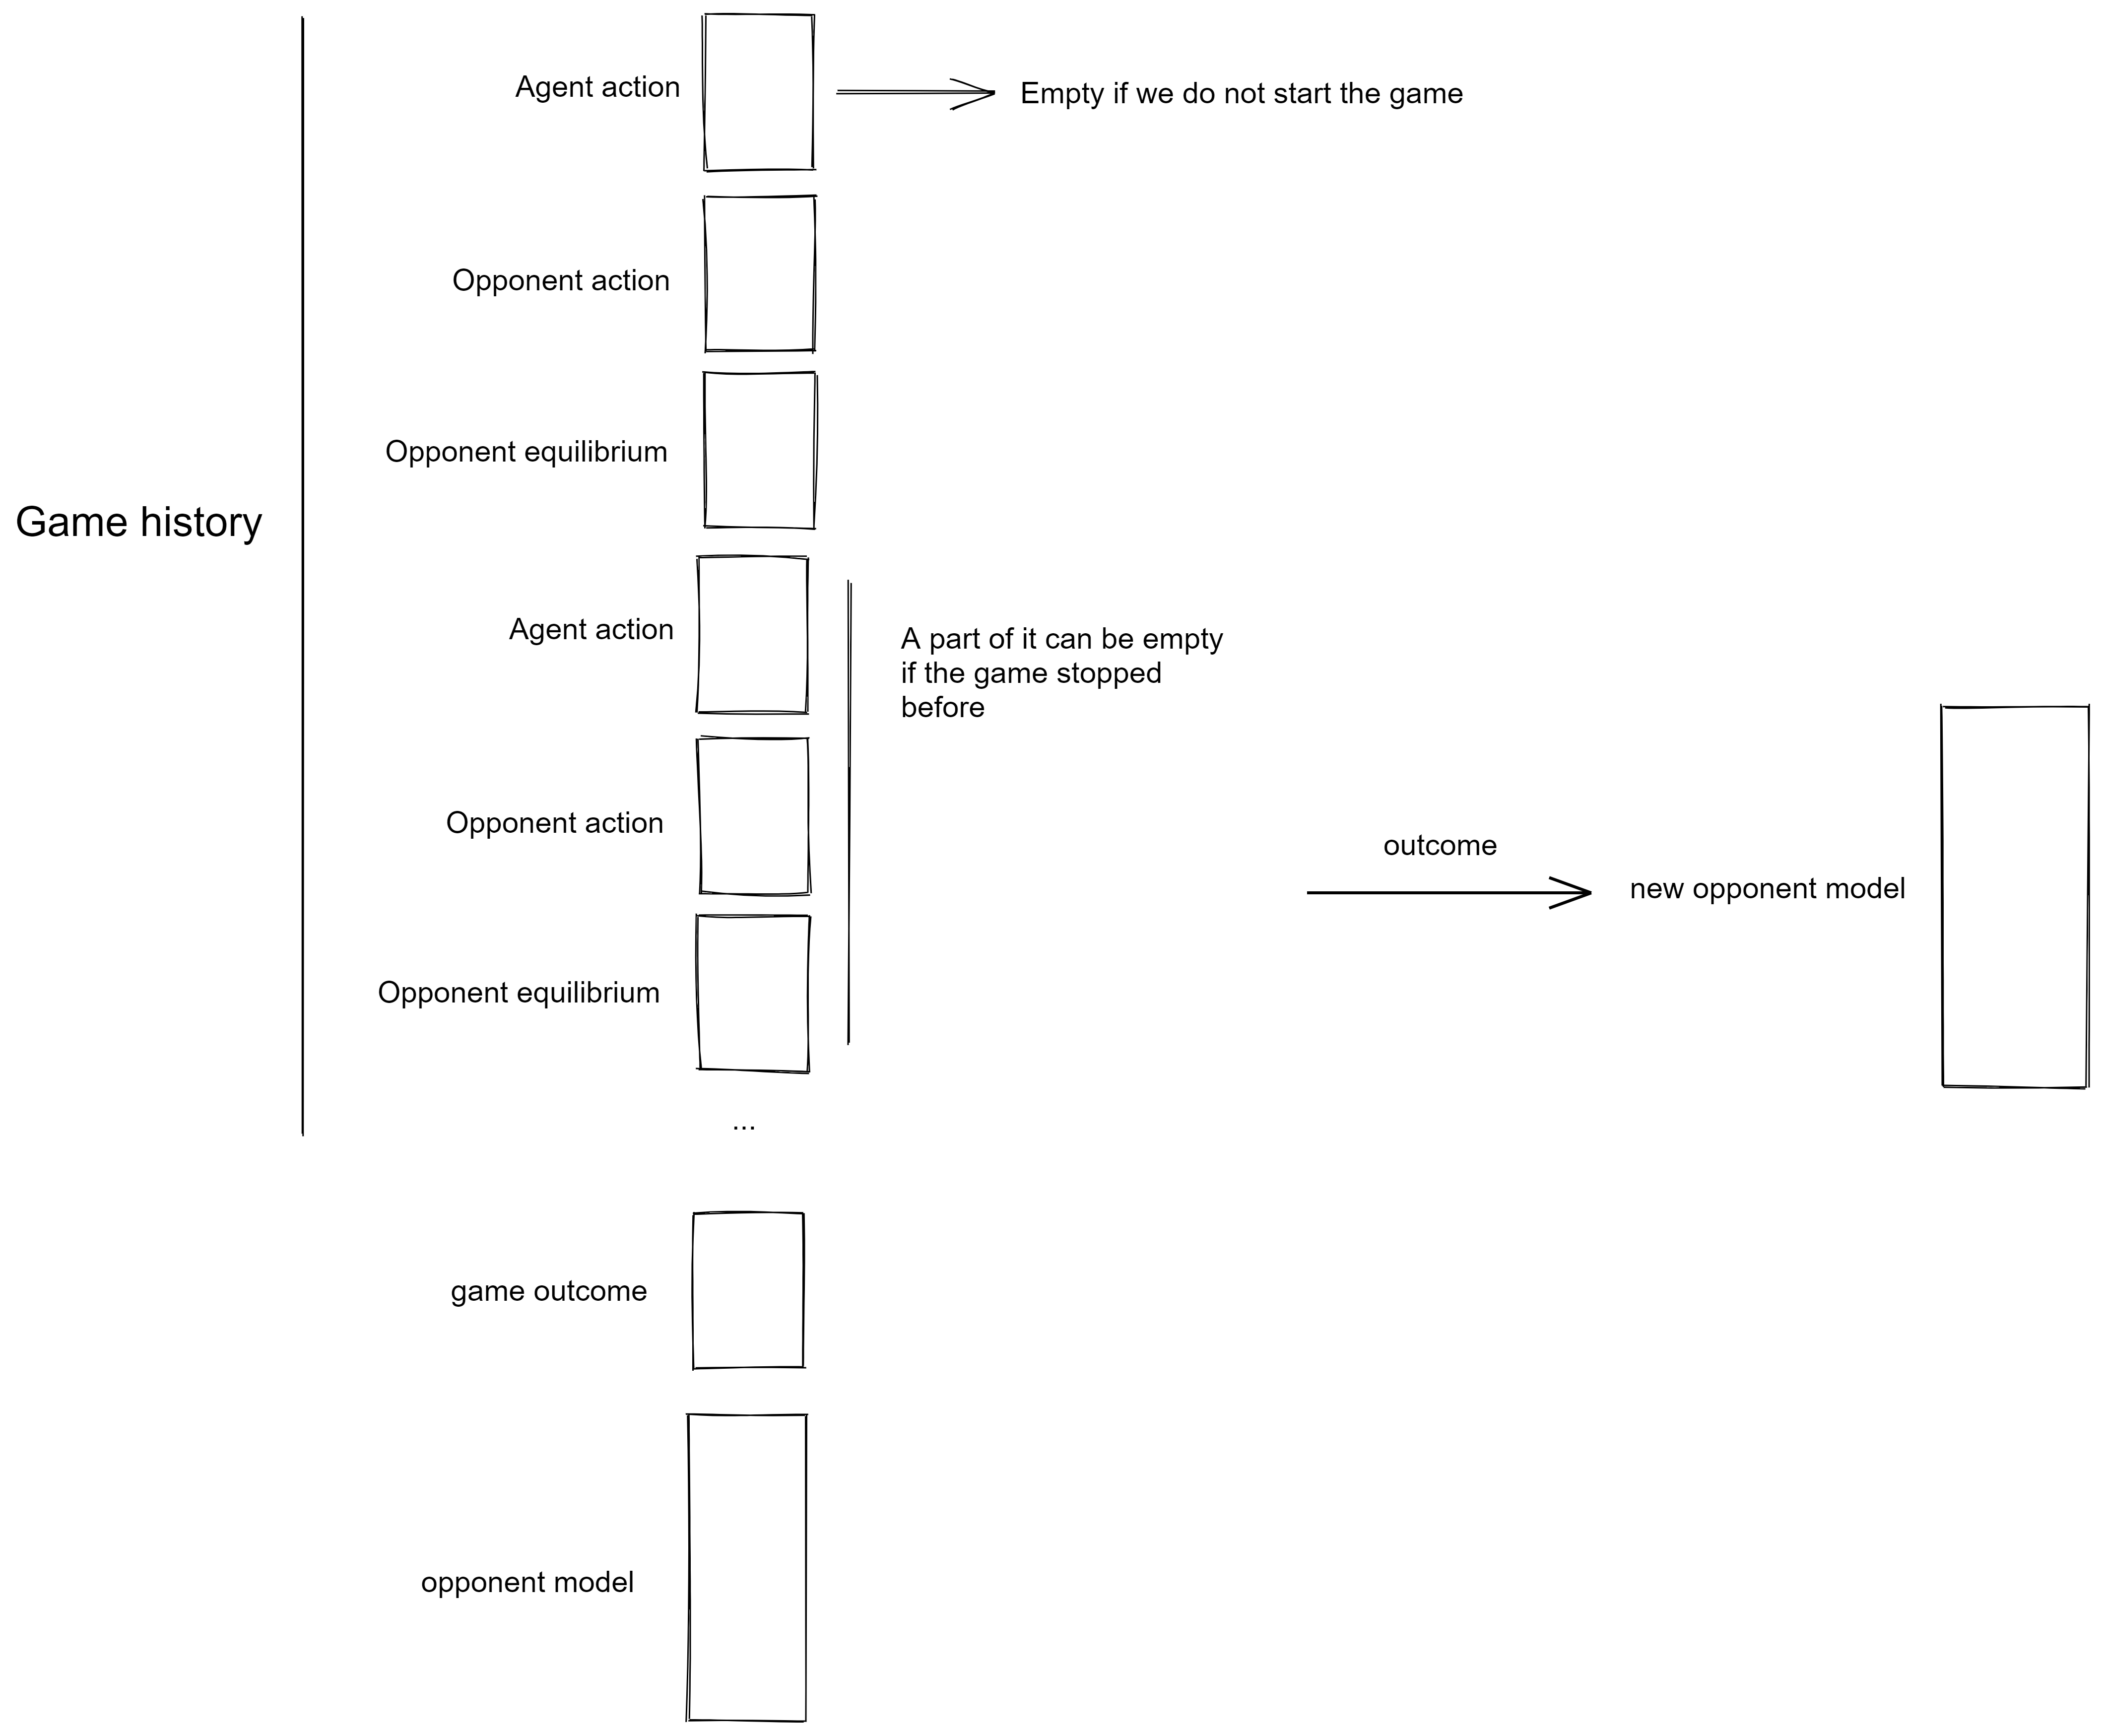
\includegraphics[width=0.9\textwidth]{Figures/opponent-modelling-nn-rnn.png}
    \caption{Opponent modelling neural network, simple RNN}
    \label{fig:opponent-modelling-nn-rnn}
\end{figure}

\begin{figure}[ht]
    \centering
    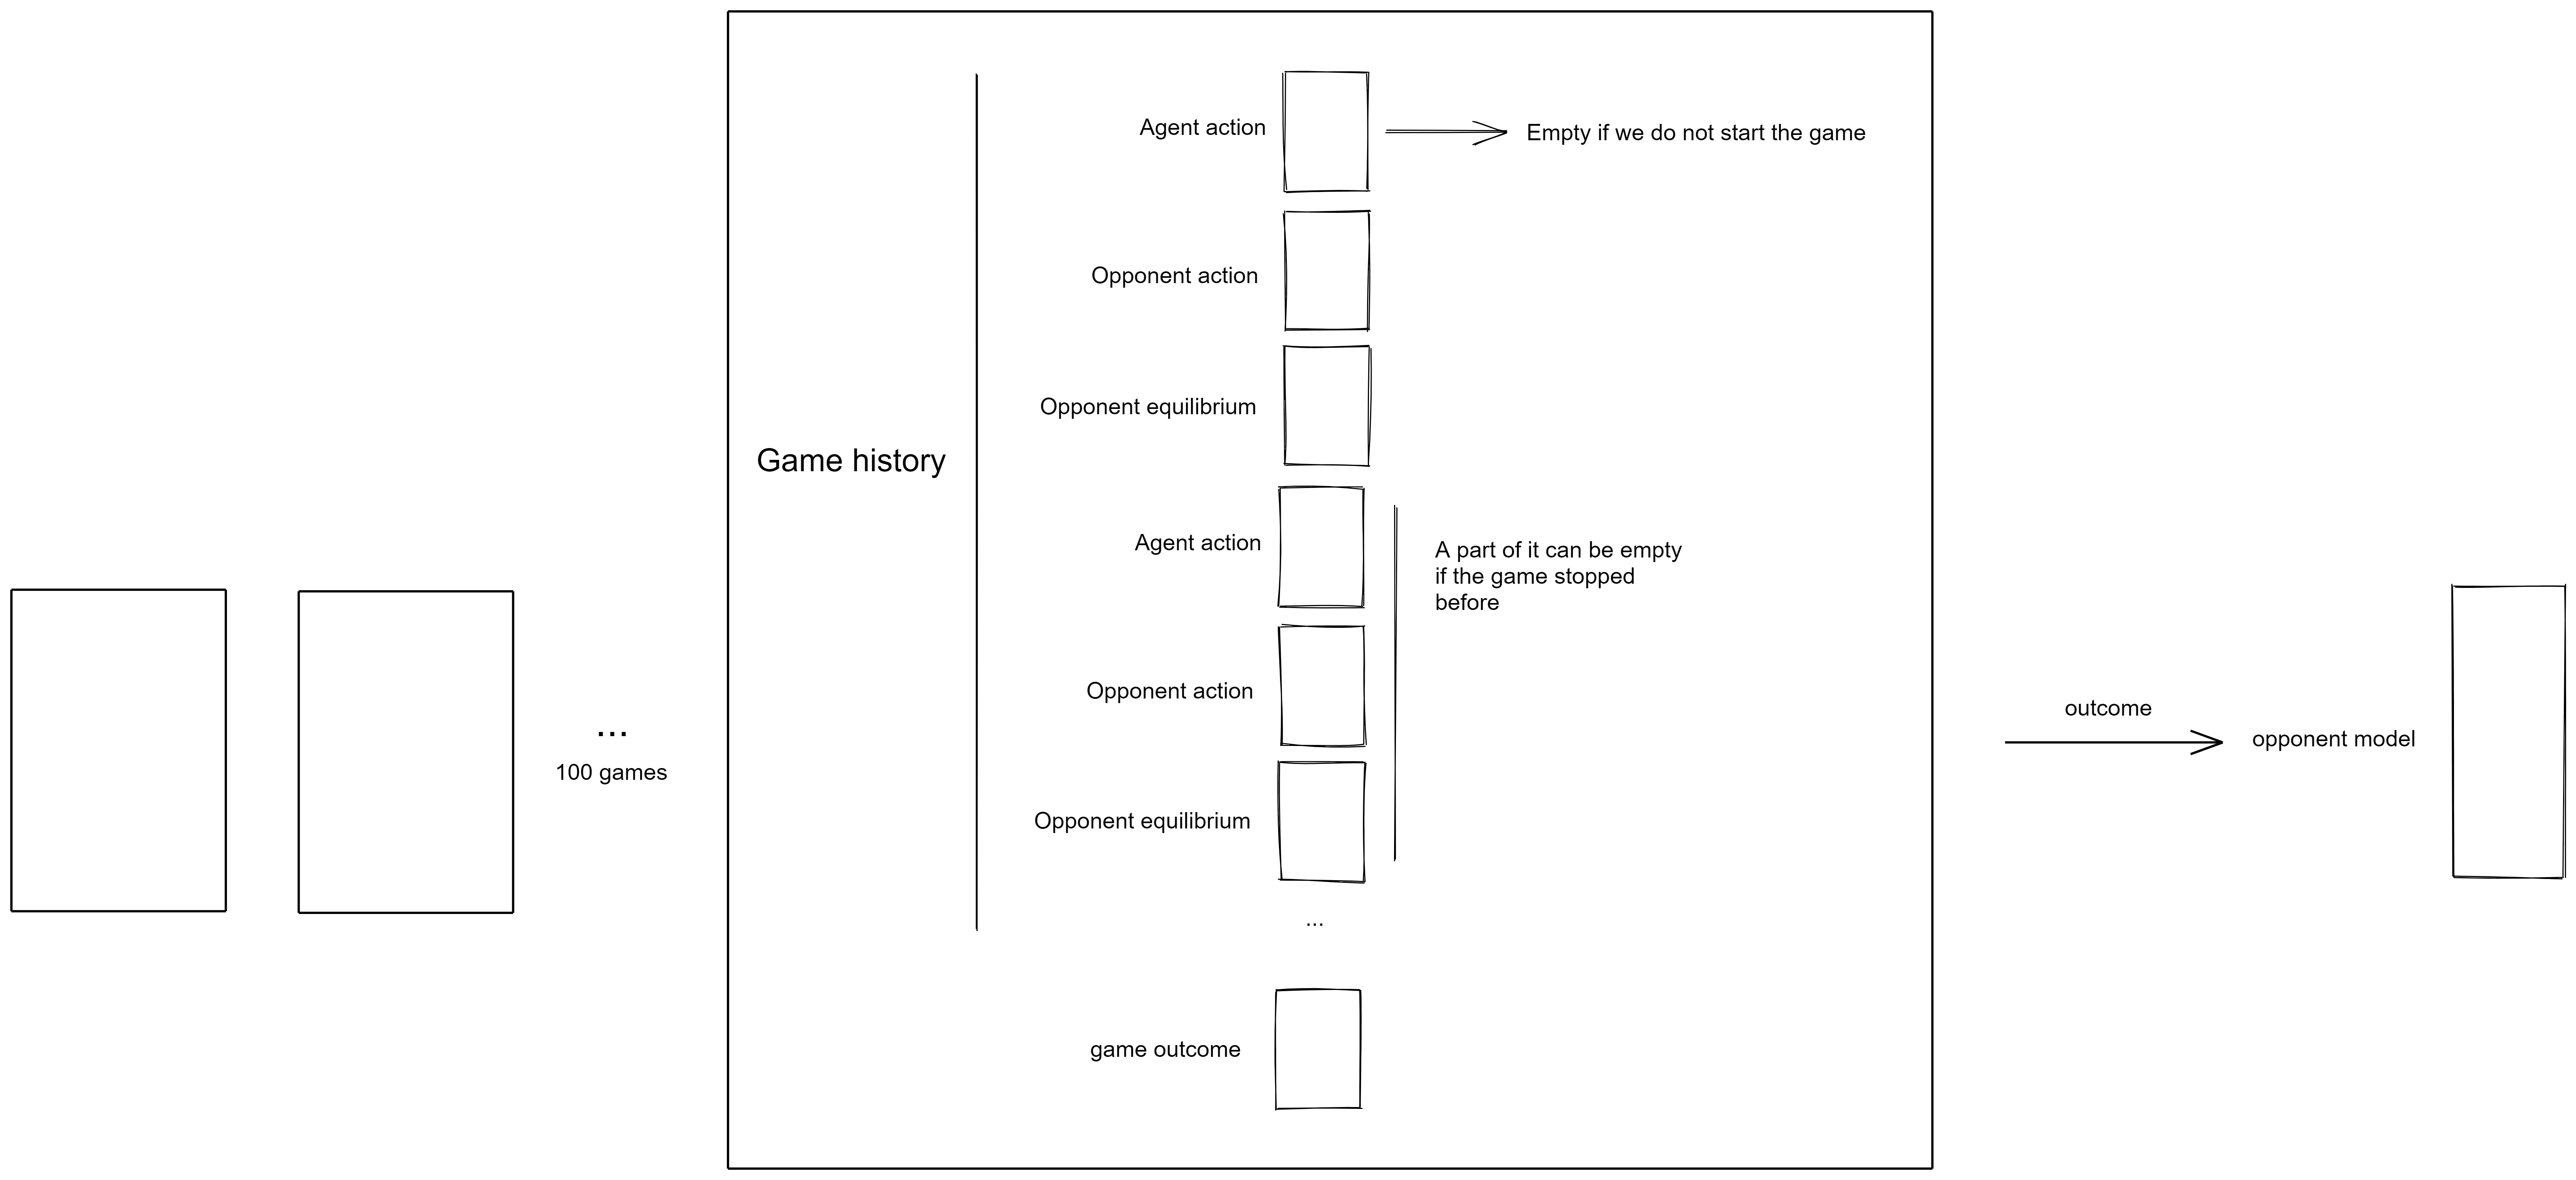
\includegraphics[width=1\textwidth]{Figures/opponent-modelling-nn-lstm.png}
    \caption{Opponent modelling neural network, LSTM kind}
    \label{fig:opponent-modelling-nn-lstm}
\end{figure}

\subsection{Decision making NN} \label{methodology:descision-making}
The decision-making NN is the one that will use the opponent model to decide which action to take within a game.

It needs to have information about the game history, we use the same representation as for the opponent modeling (section \ref{methodology:opponent-modelling:game-history}) however we do not add information about the opponent equilibrium. This might change if we see that including the global equilibrium for each agent action improve the performance.

In addition, we are giving the equilibrium of the current action for the agent. It continues the effort of feeding knowledge of the game to the NN.

You can find a schema of this neural network in figure \ref{fig:decision-making-nn}

\begin{figure}[ht]
    \centering
    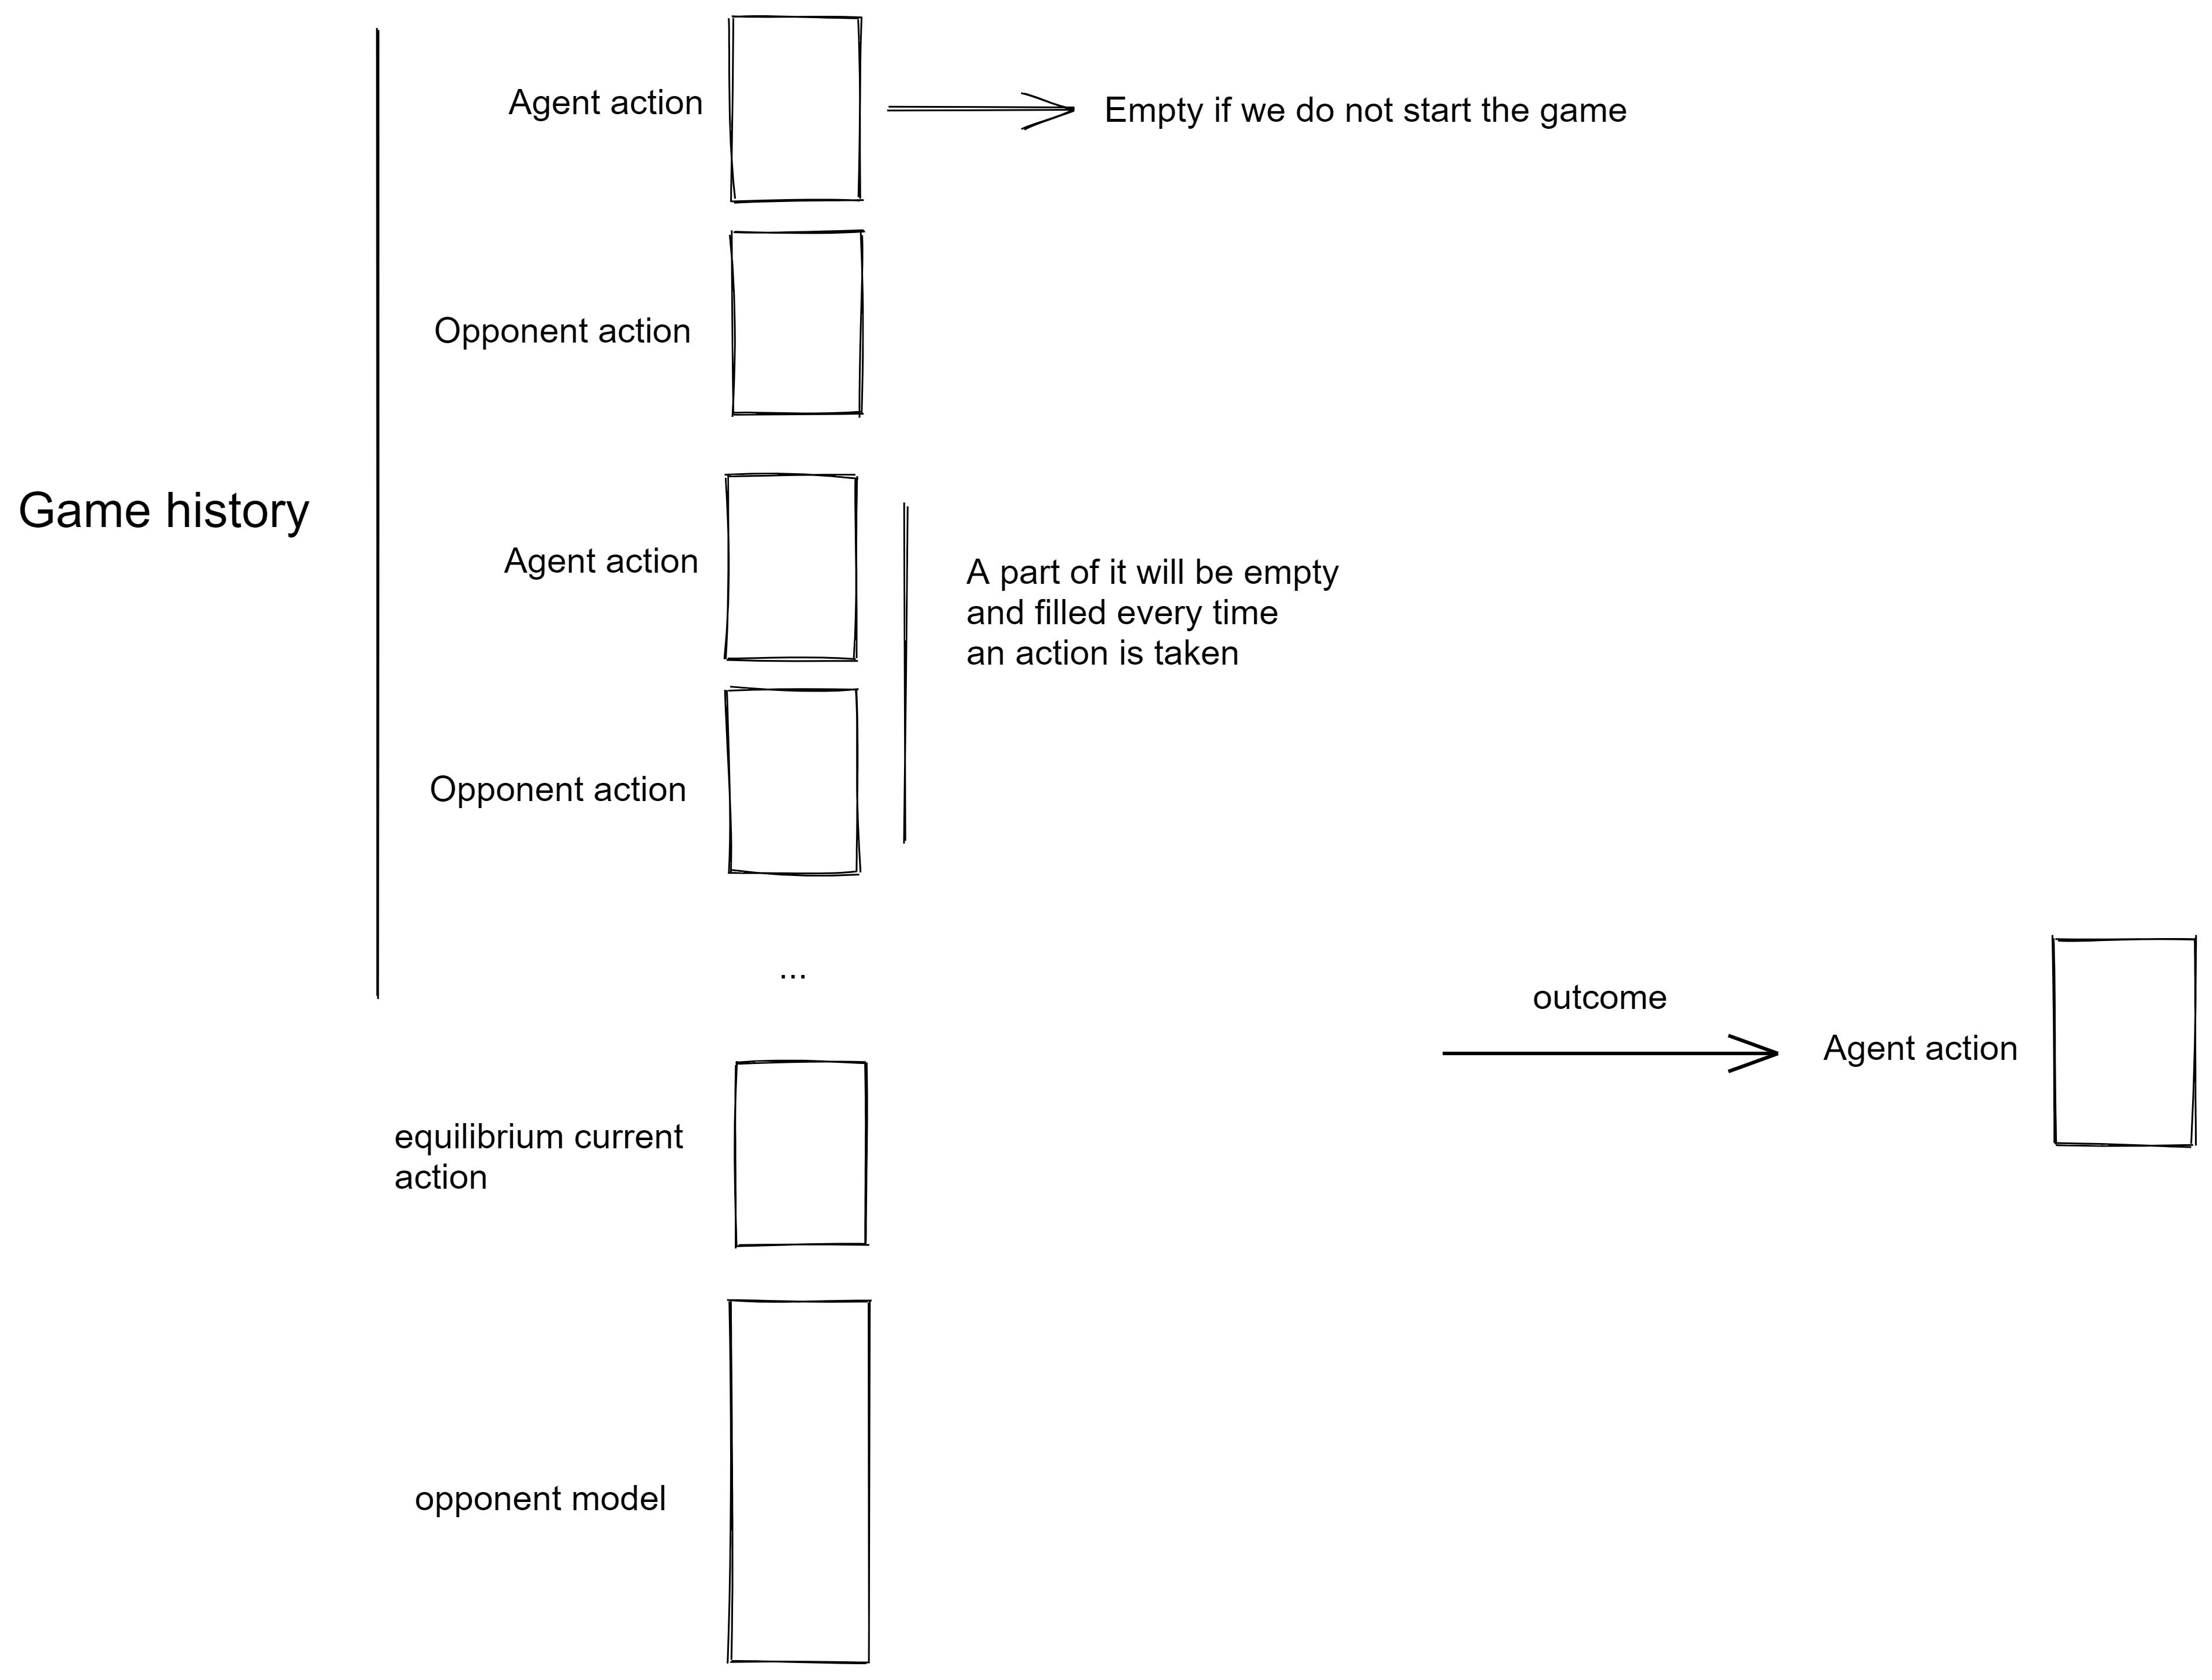
\includegraphics[width=1\textwidth]{Figures/decision-making-nn.png}
    \caption{Decision making NN}
    \label{fig:decision-making-nn}
\end{figure}

\section{Training Neural Networks}
The training of these neural networks is challenging and is the core difficulty of this project. Indeed we do not just expect our algorithm to be the best on the long term. We also expect it to be able to detect and exploit opponents.

\subsection{Attribution of reward}
We can not attribute or pre-compute the expected result given an input. Indeed the opponent modeling and decision making are too complex to calculate this. Instead, we attribute a reward given the actions taken by the agent.

The attribution of a reward is subtle and should be done carefully. We can not have a reward for every action the agent is making, it is not an instant reward.

For example, if the agent bet with bad cards maybe it is his strategy to exploit the opponent who is afraid when the agent bet. Given so we can not assign a negative reward to this action because the action takes part in a more advanced strategy. The reward needs to be given when the agent loses or wins something. In our case, if the agent ends up winning the game it will have a positive reward and a negative reward if it ends up losing the game.

It is a general idea of how attributing the reward, this can be tune given the learning algorithm used.

\subsection{Learning environment} \label{methodology:learning-environment}
The learning environment needs to make sure that the agent can learn how to exploit complex behavior. This is a difficult constraint because it means that the agent must play against multiple sub-optimal opponents.

This requires to have generated opponents created by the learning environment or/and have opponents with a fixed strategy defined before the learning starts. Having only opponents with a fixed strategy will cover only a few behaviors. Also, it makes complicated for this algorithm to be used in other imperfect game because it will require to find/create other opponents. So having only fixed strategies while learning should be avoided.

\subsection{Training algorithms}
We consider two kinds of algorithms that fit the training constraints. Competitive co-evolution and reinforcement learning.

\subsubsection{Competitive co-evolution} \label{methodology:competitive-co-evolution}
Competitive co-evolution (section: \ref{LR:competitive-co-evolution}) is the most promising kind of algorithm in its capacity of generating complex opponents and attributing a dynamic reward.

Competitive co-evolution makes multiples agents compete against each other. So it generates a set of sub-optimal opponents by design and makes it evolve into more complex agents over the training. Also, these agents start with simple behavior and the more the training continues more complex these agents became. It allows having incremental learning from simple to complex behavior.

Competitive co-evolution allows by design to have shared fitness. As said in section \ref{LR:competitive-co-evolution} it allows to promote diversity and encourage the development of promising behavior.

For evolving a NN with this algorithm, every weight needs to be encoded in a solution. Usually, EA has trouble scaling when the search space is too large. Neural networks tend to have a lot of weight, this can lead to performance issues if we are using EA to evolve it.

\subsubsection{Reinforcement Learning} \label{methodology:rl}
As said in section \ref{LR:reinforcement-learning}, reinforcement learning is made to work with rewards and have really good performance for evolving NN.

The main issue with this method is that it uses backpropagation to evolve the NN and it is hard to implement if multiple NN are involved. In our case, I think that backpropagation can be done even if we are using two NN. The reason is that a part of the decision-making input is the output of the opponent modeling NN, so we can theatrically propagate the error from one NN to the other. However, this would require extra research and work to implement it.

The second issue is that by design reinforcement learning does not work with multiple agents, in fact, it only evolves one NN. To meet our learning environment constraint (section: \ref{methodology:learning-environment}) we would need to manually find/create opponents with a fixed strategy. This is something we should avoid.

\subsection{Conclusion}
To conclude Competitive co-evolution perfectly fit the learning environment but may suffer from performance issue if the size of the NN is too important. On the other hand, reinforcement learning has really good performance for evolving NN but the solution is likely to be incomplete and suffer from a lack of diversity in the learning environment.

\section{Evaluation} \label{requirement:evaluation}
The evaluation is a crucial process for this research. It is the only way to demonstrate the capacity of neural network to model opponent behavior. Better the testing will be, the better these results will be generalized, without the need to run more experiments.

We will use poker to run our experiments. It is the most used game in imperfect game solving research as it includes complex behavior and strategy. The poker variant used will depend on the size of the game state we want to test.

Performances will be measured in milli-big blinds per hand (mbb/hand), the average number of big blinds win per 1000 hands. This is a common unit in poker research. Following this standard will allow these results to be comparable with other research papers.

\subsection{Exploitation testing} \label{requirement:evaluation:exploitation}
The exploitation testing will ensure that the algorithm successfully extracts simple opponent behavior. Even "stupid" opponents can be interesting to study because they can give metrics on how fast the algorithm exploits them.

Here is the list of the different algorithms:
\begin{itemize}
    \item Always fold
    \item Always rise
    \item Random: plays random moves
\end{itemize}

\subsection{Exploitability testing} \label{requirement:evaluation:exploitability}
Exploitability testing will provide information on how much the algorithm is exploitable.

It will play against an opponent following the equilibrium strategy. Given that, we will be able to see how reasonable our algorithm is and how well it managed to not fall into trying to exploit the equilibrium.

It will also be evaluated using the true best response with access to the private game state. In other words, at each step, the true best response will be computed with access to the card of every player. This is a non-realistic testing because it is cheating but it provides an interesting insight into how much the algorithm is exploitable.

We will also evaluate how far the algorithm is flexible and able to adapt if the opponent drastically switch his strategy. To do so we will have an opponent playing random for 100 games then playing the true best response for the remaining of the day.

\subsection{Advanced opponent testing} \label{requirement:evaluation:advanced}
In this testing category, we are trying to reproduce real-world poker examples. We will challenge our algorithm with different sub-optimal opponents.

We will use made up sub-optimal strategy by playing each action with a probability chosen uniformly randomly within 0.2 of the equilibrium probability. This type of sub-optimal opponent has been used in previous research in opponent modelling \citep{ganzfried2015safe}. It will be easier to compare the results.

We discard the usage of human testing for this research because it will require financial resources to have non-bias and conclusive results.
